\documentclass[conference]{IEEEtran}
\IEEEoverridecommandlockouts
% The preceding line is only needed to identify funding in the first footnote. If that is unneeded, please comment it out.
%Template version as of 6/27/2024

\usepackage{cite}
\usepackage{amsmath,amssymb,amsfonts}
\usepackage{algorithmic}
\usepackage{graphicx}
\usepackage{textcomp}
\usepackage{xcolor}
\usepackage{url}
\def\BibTeX{{\rm B\kern-.05em{\sc i\kern-.025em b}\kern-.08em
    T\kern-.1667em\lower.7ex\hbox{E}\kern-.125emX}}
\begin{document}

\title{Stochastic\textbackslash  Noise-Based Wireless Communication\\
%{\footnotesize \textsuperscript{*}Note: Sub-titles are not captured for https://ieeexplore.ieee.org  and should not be used}
%\thanks{Identify applicable funding agency here. If none, delete this.}
}

\author{\IEEEauthorblockN{1\textsuperscript{st} Žan Perat}
\IEEEauthorblockA{\textit{dept. name of organization (of Aff.)} \\
\textit{name of organization (of Aff.)}\\
Nova Gorica, Slovenija \\
zan.perat@gmail.com}
\and
\IEEEauthorblockN{2\textsuperscript{nd} Veljko Pejović}
\IEEEauthorblockA{\textit{dept. name of organization (of Aff.)} \\
\textit{name of organization (of Aff.)}\\
City, Country \\
email address or ORCID}
\and
\IEEEauthorblockN{3\textsuperscript{rd} Areeb Ahmed}
\IEEEauthorblockA{\textit{dept. name of organization (of Aff.)} \\
\textit{name of organization (of Aff.)}\\
City, Country \\
email address or ORCID}
}
\maketitle

\begin{abstract}
This document is a model and instructions for \LaTeX.
This and the IEEEtran.cls file define the components of your paper [title, text, heads, etc.]. *CRITICAL: Do Not Use Symbols, Special Characters, Footnotes, 
or Math in Paper Title or Abstract.
\end{abstract}

\begin{IEEEkeywords}
component, formatting, style, styling, insert.
\end{IEEEkeywords}

\section{Introduction}
Wireless communication must balance reliability, transmition time, implementation cost, and the \textbf{exposure} created by a radio emission. In military sensing and monitoring applications, transmitting short status messages may be sufficient, even when high data rates are unnecessary. In such scenarios, covert communication may be more important than high-speed data transmission, as minimizing the probability of detection can outweigh the benefits of reduced transmission time. Such settings motivate to investigate waveforms whose information is representend statistically\textbackslash stochastically rather than by a conventional deterministic symbol constellation. This work examines one of such possibility through a practical implementation and testing in some real time scenarios. 

An $\alpha$-stable random process provides a family of distributions with adjustable tail behaviour, asymmetry, scale, and location. In the communication scheme considered in this paper, the transmitter generates a new random sample sequence for each input bit.
The selected bit determines the distribution asymmetry, while the reciever recovers the bit by estimating that asymmetry from a finite sample window.
A \textbf{particular sample} value is therefore \textbf{not sufficient} to identify the transmitted bit (since it is somewhat stochastic). 
Reliability depends on the statistical evidence accumulated across the symbol. 

The use of random samples does not by itself establish confidentiality. However, noise-based waveforms have been proposed for covert communication, with prior work arguing that greater similarity between the symbol distributions makes unauthorised decoding more difficult\cite{b3}. The present study concentrates mostly on implementation, feasibility and bit error rate. At the time of writing this paper the real covertnest was still not tested. 

Moving from simulation to radio hardware itself introduces an additional set of constraints. Samples must reach the transmitter continuously (no under/overflows), the reciver must find packet boundaries (where does the noise transmittion begin end?), and independent oscillators create carrier and sampling-clock offsets. These effects are particulary important when a decoder estimates a distribution from a long window: timing errors can mix piloting simbols with data and alter statistics used for the decision.

The contributions of this paper are. First, it presents custom GNU Radio encoder and decoder blocks for binary communnication through the asymmetry ($\beta$) parameter of $\alpha$-stable noise. Second, it describes the framing, and synchronisation adaptation used to operate the simulation on two independent USRP devices that is used in this first implementation. Third, it reports simulation parameter sweeps and uncoded radio mesurements, identifying the trade-off between statistical estimator accuracy and transmition time. The contribution is an implementation and experimental evaluation of an existing modulation principle, rather than a claim to have introduced that principle.

The work relates to military communications, experimental radio systems, and the evaluation of unconventional physical layer methods. 


\section{Rationale for military application}
\subsection{Communication Use Case}
A candidate application is a low-rate link carrying a brief sensor report, equipment condition, or status update between nearby nodes. This kind of massage can tolarate a lower throughput than voice or imagery and is therefore a great candidate for lower throughput communication at hand. The relevant quetion is whether the additional observation time buys sufficient reliability to justify the longer transmission and energy expense.

The experimental platform allows that questions to be studied by changing the number of samples per symbol, the separation of the symbol distributions, the receiver estimator, and use of other statistical parameters to transmit data. SDR is useful at this early stage because these choises can be changed in software while retaining the same basic radio hardware. The present measurments establish only proof of concept. They do not establish tactical range, field reliability, or suitability for an operational deployment.

\subsection{Requirements and Evidence Needed}
For a military application, the evaluation would need to cover message delivery probability, end-to-end latency, occupied bandwith, energy per delivered message, and performance under relevant interference. If reduced detectability is an objective, an explicitly defined observer and a detection experiment are also required. Packet acquisition must be included because in this first implementation the preamble and pilot simbols are still deterministic and so can reveal a transmission even when its payload is random. In some papers the pilot problem is already addressed and is non-deterministic, that should lower the probability of detection greatly (TODO paper ask Ahmeed he said that there is already a scheem for that). 

The implemented waveform would complement higher layer protection:  authenticated encryption and replay protection would still be needed for confidentiality, integrity and message freshness (TODO idk how to say otherwise chat said to write this....). These mechanisms are outside the reported implementation, but this methods are already known and can be implemented as in existing systems. Likewise, successful decoding in additive Gausseian noise should not be interpreted as demonstrated resistence to a deliberate jammer. The military rationale is therfore a motivation for evaluating the platform under representative conditions, not an operational capability claim.

\section{Related work}
Ahmed and Savaci describe random communication based on skewed $\alpha$-stable Lévy noise shift keying \cite{b3}. Ahmed's dissertation also provides broder background on communication using $\alpha$-stable processes \cite{2}. These works form the conceptual\textbackslash matematical basis for representing symbols through distribution parameters. The focus here is the implementation of that principle in GNU Radio and the practical consequences of transferring it to independent SDR devices.

Generation and estimation are central components of such a system. The Chambers-Mallows-Stuck(CMS) method and Weron's analysis address the generation of skewed stable random variables \cite{b8}. Work by Tsihrintzis and Nikas concerns fast estimation of $\alpha$-stable parameters \cite{b20}, while Tsihrinitzis, Shao, and Nikas discuss applications and processing of stable-distributed time series \cite{b21}. These references motivate treating parameter estimation as a design choise with its own final sample limitations.

Impulsive interference is a further motivation for studying non-Gaussian models. Madi et al. examine the impact of impulsive noise on wireless performance \cite{b16}. That motivation must be distinguised from the channel used in the present simulation: here, the transmitted samples are $\alpha$-stable, but the added channel disturbance is Gaussian. The experiments do not test a seprate impulsive interferrer, that should be tested with deliberate jammer. 

An adjecent implementation direction is chaotic spread-spectrum communication on SDR \cite{b7}. Such work shares the challenge of bringing unconventional waveforms into a practical radio platform, but should not be treated as an equivalent statistical modulation scheme. The present paper contributes a concrete GNU Radio workflow and measured results for assymmetry modulation, with explicit attention to synchronization and framing overhead.

\section{Statistical modulation and receiver}
\subsection{Signal Model}
Let  $b_j\in\{0,1\}$ denote the $j$-th payload bit. The binary mapping is:
\begin{equation}
$\beta_j = (2b_j - 1) \frac{\Delta \beta}{2}$,
\end{equation}
where $0<\Delta\beta\leq2$ controls the separation of the two distributions. The largest separation gives $\beta_j\in\{-1,1\}$. The transmitter generates $N$ independent samples per bit,
\begin{equation}
$x_{j,k}\sim S_\alpha(\beta_j,\gamma,0),\quad k=1,\ldots,N$.
\end{equation}
In this implementation information is encoded exclusively through $\beta$, but other parameters are open for further implementation.


For the simulated additive channel,
\begin{equation}
$y_{j,k}=x_{j,k}+w_{j,k}$,
\end{equation}
where $w_{j,k}$ is Gaussian noise. This is a simulation model, not a complete model of the physical radio link. Hardware transmission additionally introduces gain, filtering, finite dynamic range, carrier offsets, and timing uncertainty.

The parameter $\alpha$ controls tail behaviour, $\beta$ controls asymmetry, and $\gamma$ controls scale. For $\alpha<2$, an ideal stable variable has no finite second moment. Consequently, a conventional signal-power interpretation requires care. Moreover, finite radio hardware cannot reproduce unbounded tails (hardware has limmitations you clip to max min...). The mapping from generated samples to the transmitted amplitude range is therefore an important item to document and control in subsequent measurements.







\subsection{Units}
\begin{itemize}
\item Use either SI (MKS) or CGS as primary units. (SI units are encouraged.) English units may be used as secondary units (in parentheses). An exception would be the use of English units as identifiers in trade, such as ``3.5-inch disk drive''.
\item Avoid combining SI and CGS units, such as current in amperes and magnetic field in oersteds. This often leads to confusion because equations do not balance dimensionally. If you must use mixed units, clearly state the units for each quantity that you use in an equation.
\item Do not mix complete spellings and abbreviations of units: ``Wb/m\textsuperscript{2}'' or ``webers per square meter'', not ``webers/m\textsuperscript{2}''. Spell out units when they appear in text: ``. . . a few henries'', not ``. . . a few H''.
\item Use a zero before decimal points: ``0.25'', not ``.25''. Use ``cm\textsuperscript{3}'', not ``cc''.)
\end{itemize}

\subsection{Equations}
Number equations consecutively. To make your 
equations more compact, you may use the solidus (~/~), the exp function, or 
appropriate exponents. Italicize Roman symbols for quantities and variables, 
but not Greek symbols. Use a long dash rather than a hyphen for a minus 
sign. Punctuate equations with commas or periods when they are part of a 
sentence, as in:
\begin{equation}
a+b=\gamma\label{eq}
\end{equation}

Be sure that the 
symbols in your equation have been defined before or immediately following 
the equation. Use ``\eqref{eq}'', not ``Eq.~\eqref{eq}'' or ``equation \eqref{eq}'', except at 
the beginning of a sentence: ``Equation \eqref{eq} is . . .''

\subsection{\LaTeX-Specific Advice}

Please use ``soft'' (e.g., \verb|\eqref{Eq}|) cross references instead
of ``hard'' references (e.g., \verb|(1)|). That will make it possible
to combine sections, add equations, or change the order of figures or
citations without having to go through the file line by line.

Please don't use the \verb|{eqnarray}| equation environment. Use
\verb|{align}| or \verb|{IEEEeqnarray}| instead. The \verb|{eqnarray}|
environment leaves unsightly spaces around relation symbols.

Please note that the \verb|{subequations}| environment in {\LaTeX}
will increment the main equation counter even when there are no
equation numbers displayed. If you forget that, you might write an
article in which the equation numbers skip from (17) to (20), causing
the copy editors to wonder if you've discovered a new method of
counting.

{\BibTeX} does not work by magic. It doesn't get the bibliographic
data from thin air but from .bib files. If you use {\BibTeX} to produce a
bibliography you must send the .bib files. 

{\LaTeX} can't read your mind. If you assign the same label to a
subsubsection and a table, you might find that Table I has been cross
referenced as Table IV-B3. 

{\LaTeX} does not have precognitive abilities. If you put a
\verb|\label| command before the command that updates the counter it's
supposed to be using, the label will pick up the last counter to be
cross referenced instead. In particular, a \verb|\label| command
should not go before the caption of a figure or a table.

Do not use \verb|\nonumber| inside the \verb|{array}| environment. It
will not stop equation numbers inside \verb|{array}| (there won't be
any anyway) and it might stop a wanted equation number in the
surrounding equation.

\subsection{Some Common Mistakes}\label{SCM}
\begin{itemize}
\item The word ``data'' is plural, not singular.
\item The subscript for the permeability of vacuum $\mu_{0}$, and other common scientific constants, is zero with subscript formatting, not a lowercase letter ``o''.
\item In American English, commas, semicolons, periods, question and exclamation marks are located within quotation marks only when a complete thought or name is cited, such as a title or full quotation. When quotation marks are used, instead of a bold or italic typeface, to highlight a word or phrase, punctuation should appear outside of the quotation marks. A parenthetical phrase or statement at the end of a sentence is punctuated outside of the closing parenthesis (like this). (A parenthetical sentence is punctuated within the parentheses.)
\item A graph within a graph is an ``inset'', not an ``insert''. The word alternatively is preferred to the word ``alternately'' (unless you really mean something that alternates).
\item Do not use the word ``essentially'' to mean ``approximately'' or ``effectively''.
\item In your paper title, if the words ``that uses'' can accurately replace the word ``using'', capitalize the ``u''; if not, keep using lower-cased.
\item Be aware of the different meanings of the homophones ``affect'' and ``effect'', ``complement'' and ``compliment'', ``discreet'' and ``discrete'', ``principal'' and ``principle''.
\item Do not confuse ``imply'' and ``infer''.
\item The prefix ``non'' is not a word; it should be joined to the word it modifies, usually without a hyphen.
\item There is no period after the ``et'' in the Latin abbreviation ``et al.''.
\item The abbreviation ``i.e.'' means ``that is'', and the abbreviation ``e.g.'' means ``for example''.
\end{itemize}
% Removed the template-only citation to the sample reference b7.

\subsection{Authors and Affiliations}\label{AAA}
\textbf{The class file is designed for, but not limited to, six authors.} A 
minimum of one author is required for all conference articles. Author names 
should be listed starting from left to right and then moving down to the 
next line. This is the author sequence that will be used in future citations 
and by indexing services. Names should not be listed in columns nor group by 
affiliation. Please keep your affiliations as succinct as possible (for 
example, do not differentiate among departments of the same organization).

\subsection{Identify the Headings}\label{ITH}
Headings, or heads, are organizational devices that guide the reader through 
your paper. There are two types: component heads and text heads.

Component heads identify the different components of your paper and are not 
topically subordinate to each other. Examples include Acknowledgments and 
References and, for these, the correct style to use is ``Heading 5''. Use 
``figure caption'' for your Figure captions, and ``table head'' for your 
table title. Run-in heads, such as ``Abstract'', will require you to apply a 
style (in this case, italic) in addition to the style provided by the drop 
down menu to differentiate the head from the text.

Text heads organize the topics on a relational, hierarchical basis. For 
example, the paper title is the primary text head because all subsequent 
material relates and elaborates on this one topic. If there are two or more 
sub-topics, the next level head (uppercase Roman numerals) should be used 
and, conversely, if there are not at least two sub-topics, then no subheads 
should be introduced.

\subsection{Figures and Tables}\label{FAT}
\paragraph{Positioning Figures and Tables} Place figures and tables at the top and 
bottom of columns. Avoid placing them in the middle of columns. Large 
figures and tables may span across both columns. Figure captions should be 
below the figures; table heads should appear above the tables. Insert 
figures and tables after they are cited in the text. Use the abbreviation 
``Fig.~\ref{fig}'', even at the beginning of a sentence.

\begin{table}[htbp]
\caption{Table Type Styles}
\begin{center}
\begin{tabular}{|c|c|c|c|}
\hline
\textbf{Table}&\multicolumn{3}{|c|}{\textbf{Table Column Head}} \\
\cline{2-4} 
\textbf{Head} & \textbf{\textit{Table column subhead}}& \textbf{\textit{Subhead}}& \textbf{\textit{Subhead}} \\
\hline
copy& More table copy$^{\mathrm{a}}$& &  \\
\hline
\multicolumn{4}{l}{$^{\mathrm{a}}$Sample of a Table footnote.}
\end{tabular}
\label{tab1}
\end{center}
\end{table}

\begin{figure}[htbp]
\centerline{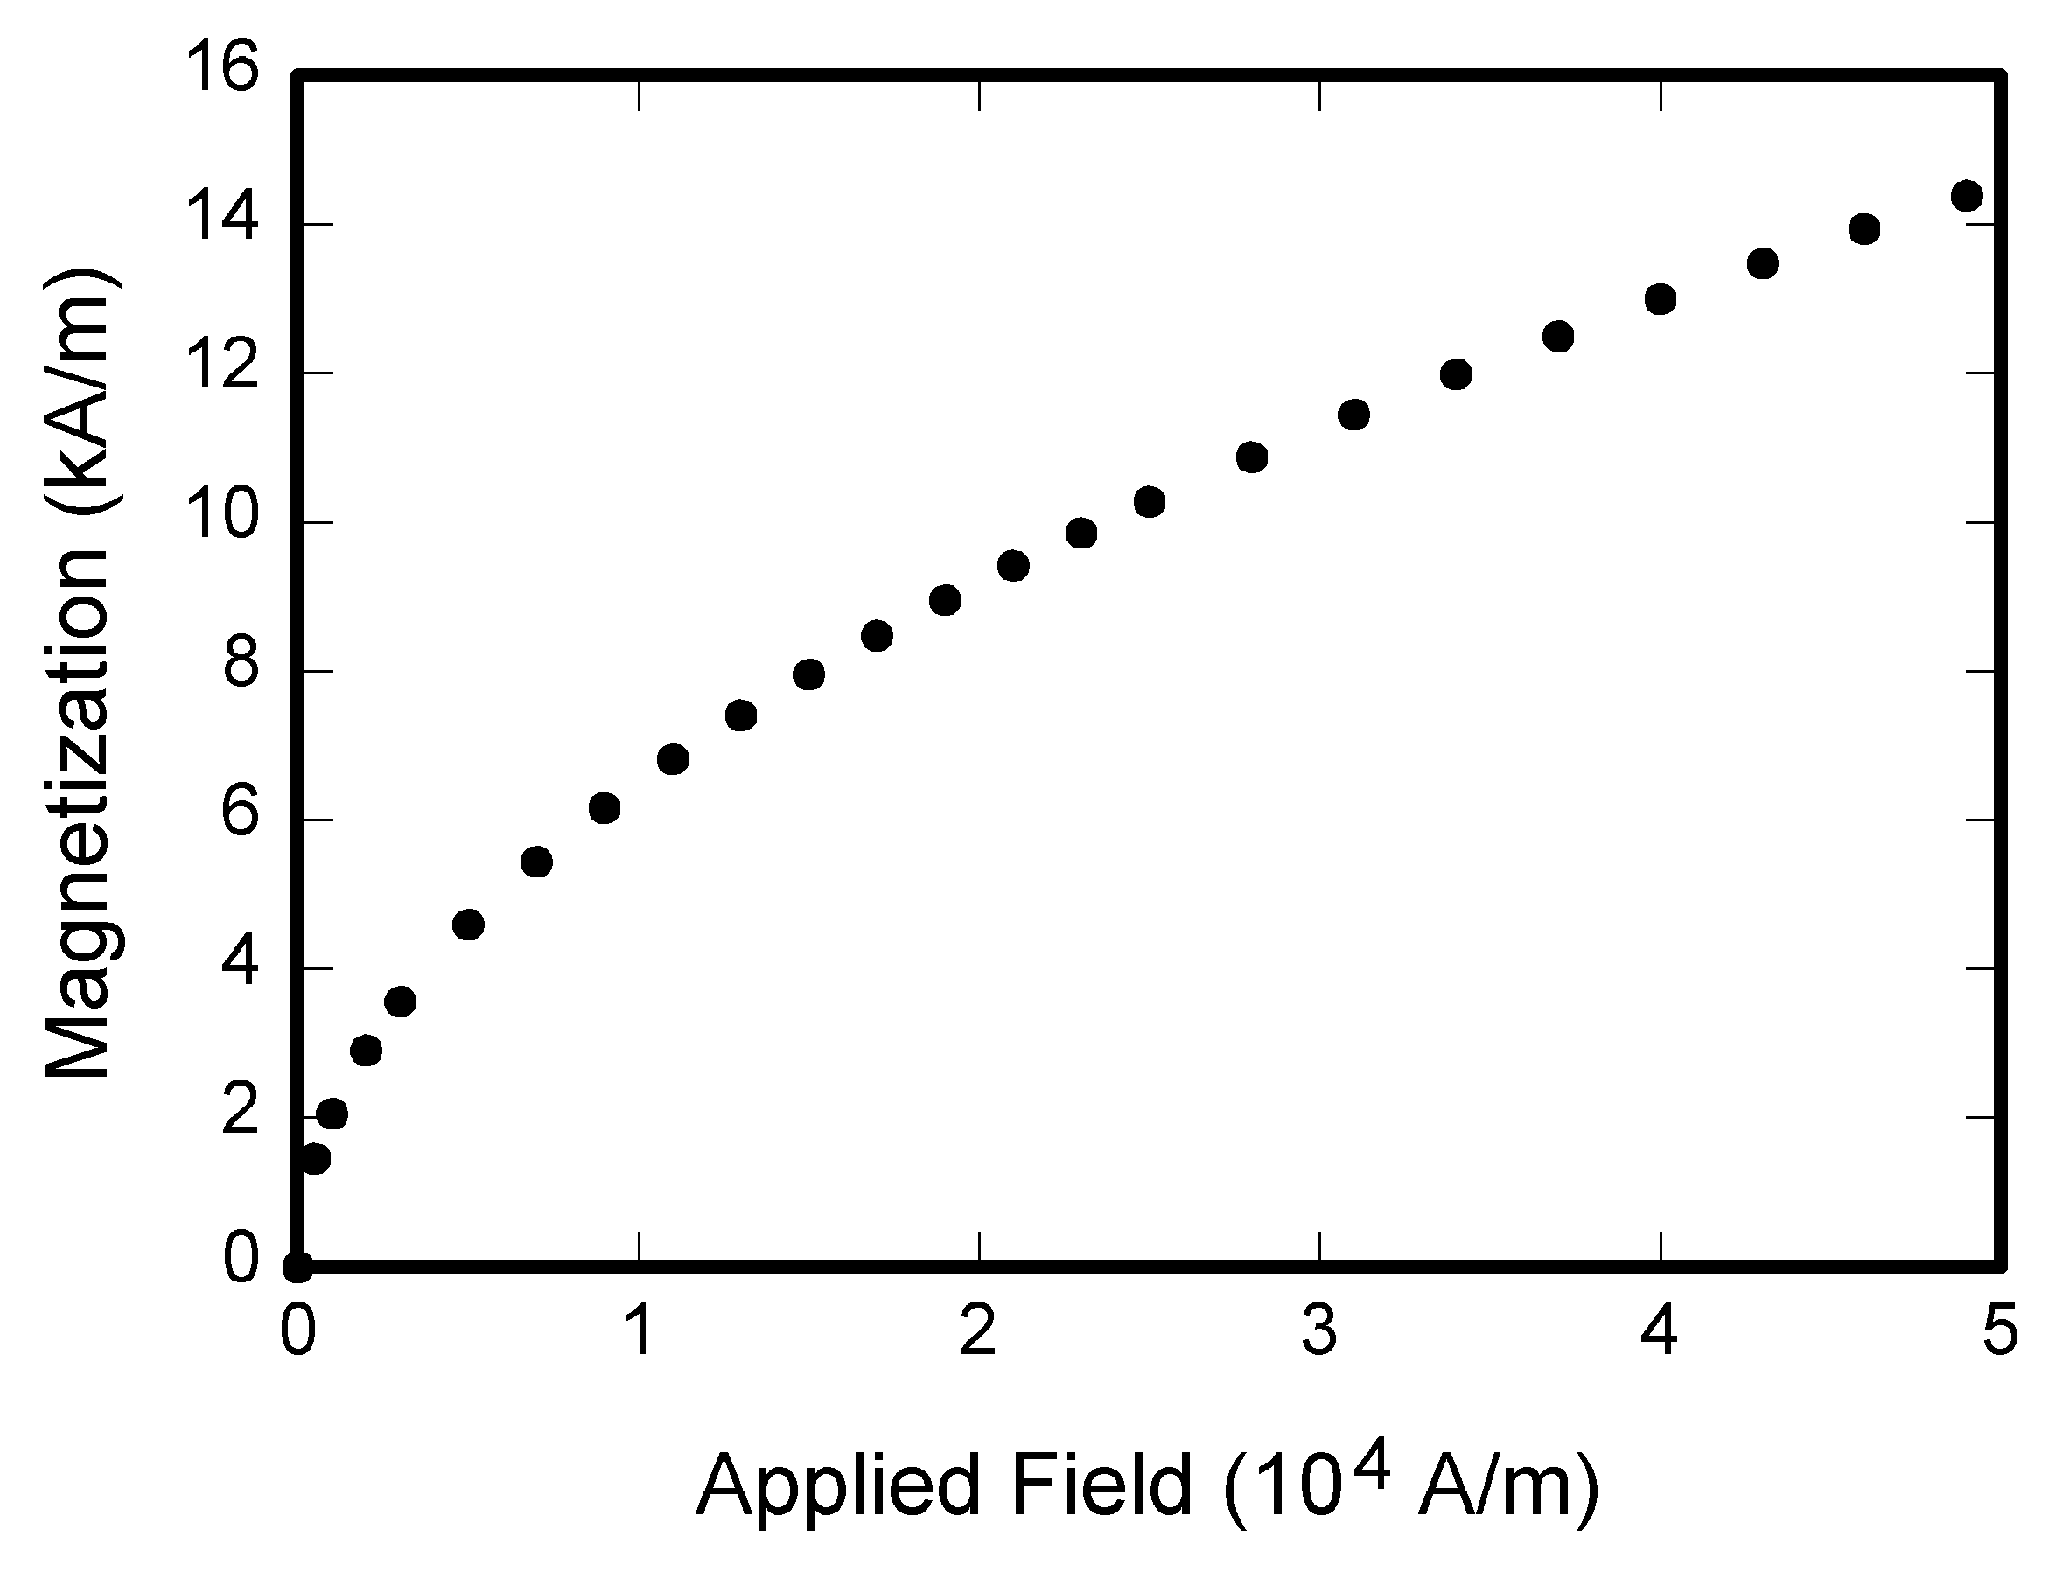
\includegraphics{fig1.png}}
\caption{Example of a figure caption.}
\label{fig}
\end{figure}

Figure Labels: Use 8 point Times New Roman for Figure labels. Use words 
rather than symbols or abbreviations when writing Figure axis labels to 
avoid confusing the reader. As an example, write the quantity 
``Magnetization'', or ``Magnetization, M'', not just ``M''. If including 
units in the label, present them within parentheses. Do not label axes only 
with units. In the example, write ``Magnetization (A/m)'' or ``Magnetization 
\{A[m(1)]\}'', not just ``A/m''. Do not label axes with a ratio of 
quantities and units. For example, write ``Temperature (K)'', not 
``Temperature/K''.

\section*{Acknowledgment}

The preferred spelling of the word ``acknowledgment'' in America is without 
an ``e'' after the ``g''. Avoid the stilted expression ``one of us (R. B. 
G.) thanks $\ldots$''. Instead, try ``R. B. G. thanks$\ldots$''. Put sponsor 
acknowledgments in the unnumbered footnote on the first page.

\begin{thebibliography}{00}
\bibitem{b1} {Statistics How To}, ``Alpha stable distribution,'' Available at: \url{https://www.statisticshowto.com/alpha-stable-distribution/}, n.d.
\bibitem{b2} {Wikipedia}, ``Stable distribution,'' Available at: \url{https://en.wikipedia.org/wiki/Stable_distribution}, 2026.
\bibitem{b3} A. Ahmed and F. A. Savaci, ``Random communication system based on skewed alpha-stable levy noise shift keying,'' Journal of Circuits, Systems and Computers, vol. 26, no. 11, p. 1750186, 2017.
\bibitem{b4} A. Ahmed, ``Random communication systems based on alpha-stable processes,'' Doctoral dissertation, Graduate School of Engineering and Sciences, Izmir Institute of Technology, Izmir, Turkey, 2018.
\bibitem{b5} {Ettus Research}, ``{USRP B210 USB Software Defined Radio (SDR)},'' Available at: \url{https://www.ettus.com/all-products/ub210-kit/}, 2026.
\bibitem{b6} {WA5VJB}, ``{850--6500 MHz PCB LP Antenna LP8565A2},'' Available at: \url{https://www.wa5vjb.com/pcb-pdfs/LP8565A2.pdf}, 2012.
\bibitem{b7} A. Aboltins, F. Capligins, N. Hasjuks, and A. Ahrens, ``Implementation of chaotic frequency modulation based spread spectrum communication system in software-defined radio,'' in 2019 Open Conference of Electrical, Electronic and Information Sciences (eStream). IEEE, 2019, pp. 1--4.
\bibitem{b8} R. Weron, ``On the {Chambers--Mallows--Stuck} method for simulating skewed stable random variables,'' Statistics \& Probability Letters, vol. 28, no. 2, pp. 165--171, 1996.
\bibitem{b9} V. Lutovac and E. Kočan, ``Physical layer security in wireless networks -- concept, performance and perspectives,'' in Proceedings of the 29th International Conference on Information Technology (IT). IEEE, 2025.
\bibitem{b10} {Wikipedia}, ``Additive white gaussian noise,'' Available at: \url{https://en.wikipedia.org/wiki/Additive_white_Gaussian_noise}, 2026.
\bibitem{b11} {IB-Lenhardt AG}, ``Awgn (additive white gaussian noise) -- definition and use,'' Available at: \url{https://ib-lenhardt.com/kb/glossary/awgn}, 2025.
\bibitem{b12} {Bluetooth Special Interest Group}, ``How bluetooth technology uses adaptive frequency hopping to overcome packet interference,'' Available at: \url{https://www.bluetooth.com/blog/how-bluetooth-technology-uses-adaptive-frequency-hopping-to-overcome-packet-interference/}, 2020.
\bibitem{b13} {Wikipedia}, ``Cauchy distribution,'' Available at: \url{https://en.wikipedia.org/wiki/Cauchy_distribution}, 2026.
\bibitem{b14} {Wikipedia}, ``Normal distribution,'' Available at: \url{https://en.wikipedia.org/wiki/Normal_distribution}, 2026.
\bibitem{b15} {GNU Radio}, ``Noise source,'' Available at: \url{https://wiki.gnuradio.org/index.php/Noise_Source}, 2025.
\bibitem{b16} G. Madi, F. Sacuto, B. Vrigneau, B. L. Agba, Y. Pousset, R. Vauzelle, and F. Gagnon, ``Impacts of impulsive noise from partial discharges on wireless systems performance: application to mimo precoders,'' EURASIP Journal on Wireless Communications and Networking, vol. 2011, no. 186, 2011.
\bibitem{b17} {GNU Radio}, ``Gnu radio,'' Available at: \url{https://www.gnuradio.org/}, 2026.
\bibitem{b18} R. M. Balan, ``Spdes with {${\alpha}$}-stable {L{\'e}vy} noise: A random field approach,'' International Journal of Stochastic Analysis, vol. 2014, no. 1, p. 793275, 2014.
\bibitem{b19} X. Liu and A. Goldsmith, ``Wireless communication tradeoffs in distributed control,'' in Proceedings of the 42nd IEEE Conference on Decision and Control, vol. 1. Maui, HI, USA: IEEE, 2003, pp. 688--694.
\bibitem{b20} G. A. Tsihrintzis and C. L. Nikias, ``Fast estimation of the parameters of {Alpha-Stable} impulsive interference,'' Signal and Image Processing Institute, University of Southern California, Los Angeles, CA, USA, Tech. Rep. USC-SIPI Report 270, Sep. 1994.
\bibitem{b21} G. A. Tsihrintzis, M. Shao, and C. L. Nikias, ``Recent results in applications and processing of {${\alpha}$}-stable-distributed time series,'' Journal of the Franklin Institute, vol. 333, no. 4, pp. 467--497, Jul. 1996.
\end{thebibliography}

\end{document}

